\documentclass[10pt,a4paper]{ctexart}
\usepackage[margin=2cm]{geometry}
\usepackage{graphicx}
\usepackage{hyperref}
\usepackage{amsmath}    % 提供方程环境
\usepackage{amssymb} 
\usepackage{physics}    % 简化向量、微分算子语法
\newcommand{\myspace}[1]{\par\vspace{#1\baselineskip}} %自定义空一行
\usepackage{fancyhdr}
\usepackage{wrapfig}
\usepackage{multirow}
\usepackage{booktabs} % 添加 booktabs 宏包
\usepackage{float}
\usepackage{subcaption}
\pagestyle{fancy}
\fancyhf{}  % 清除所有页眉页脚
\fancyfoot[C]{\thepage}  % 在页脚中央设置页码253696
\renewcommand{\headrulewidth}{0pt}  % 去掉页眉横线
\renewcommand{\footrulewidth}{0pt}  % 去掉页脚横线
% hyperref 已在上方加载一次，避免重复加载
\hypersetup{
    colorlinks=true,
    linkcolor=blue,
    filecolor=magenta,      
    urlcolor=cyan,
    pdftitle={Overleaf Example},
    pdfpagemode=FullScreen,
    }

\usepackage{titlesec}

% 重新定义section格式
\titleformat{\section}
  {\normalfont\Large\bfseries}
  {\chinese{section}、}
  {0pt}
  {}

% 给出常用字号的自定义指令
\newcommand{\chuhao}{\fontsize{42pt}{48pt}\selectfont}
\newcommand{\xiaochu}{\fontsize{36pt}{42pt}\selectfont}
\newcommand{\xiaoer}{\fontsize{18pt}{21.6pt}\selectfont}
\newcommand{\sanhao}{\fontsize{16pt}{20pt}\selectfont}
\newcommand{\xiaosan}{\fontsize{15pt}{18pt}\selectfont}
\newcommand{\sihao}{\fontsize{14pt}{18pt}\selectfont}
\newcommand{\xiaosi}{\fontsize{12pt}{16pt}\selectfont}
\newcommand{\wuhao}{\fontsize{ 10.5pt}{12.6pt}\selectfont}

% 定义中文数字转换
\titleformat{\section}
  {\normalfont\Large\bfseries}
  {\zhnum{section}、}  % 使用\zhnum而不是\chinese
  {0pt}
  {}

% 标题设置
\title{\xiaochu\textbf{物理实验报告}}
\author{}
\date{}

\begin{document}

\vspace*{36pt} % 顶部空白

% 居中填写区域
\begin{center}
    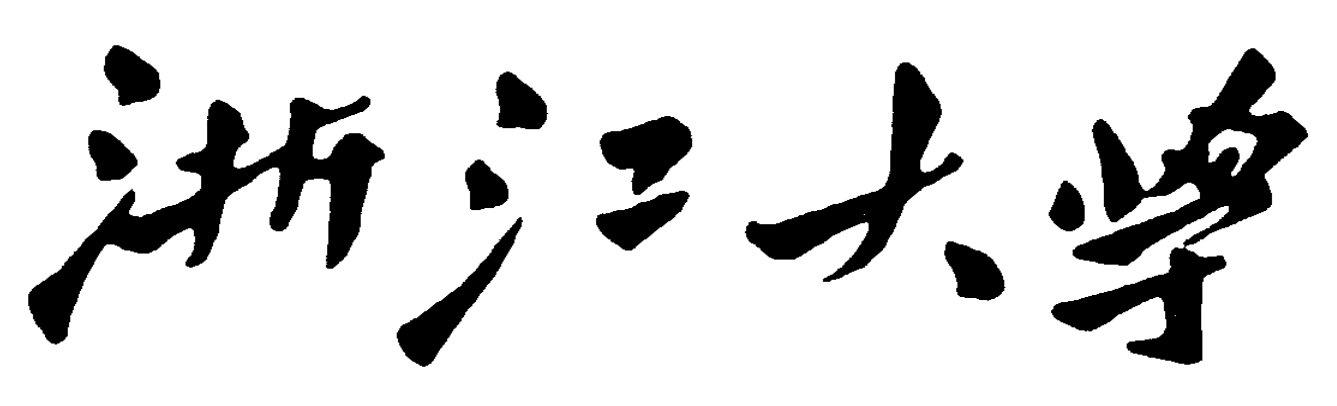
\includegraphics[width = 9cm]{figures/head.png}
    
    \xiaochu\textbf{物理实验报告}
    % 预留空白区域
    \vspace{13pt}
    \vspace{13pt}
    \vspace{13pt}
    \vspace{13pt}
    
    \sanhao\textbf{实验名称：\underline{\makebox[11cm]{ 声速的测定 }}} \\[10pt]
    \sanhao\textbf{实验桌号：\underline{\makebox[8cm]{ }}} \\[10pt]
    \sanhao\textbf{指导教师：\underline{\makebox[8cm]{  }}} \\[20pt]
    
    % 预留空白区域
    \myspace{7}
    
   \sihao\textbf{班级：\underline{\makebox[6cm]{cc98}}} \\[10pt]
    \sihao\textbf{姓名：\underline{\makebox[6cm]{Hydrofoil}}} \\[10pt]
    \sihao\textbf{学号：\underline{\makebox[6cm]{324010}}} \\[30pt]
    
    \sihao\textbf{实验日期: \underline{\makebox[0.8cm]{2025}}年 \underline{\makebox[0.4cm]{12}}月\underline{\makebox[0.4cm]{24}}日  星期\underline{\makebox[0.6cm]{三}}上午}
    
    \vspace{18pt}
    \sihao 浙江大学物理实验教学中心
    
\end{center}

\newpage

\section{预习报告}


    \subsection{实验综述}  

    \xiaosi （自述实验现象、实验原理和实验方法，不超过500字，5分）

    \subsubsection*{实验原理}

    \textbf{超声波传播速度：}声波在理想气体中传播可看作绝热过程。其传播速度 $V = \sqrt{\frac{\gamma RT}{M}}$ （其中，$M$为气体摩尔质量，$R$为摩尔气体常量，$\gamma$为气体的比热容比，$T$为气体的热力学温度）。 在 $0^{\circ}C$ 时，声速 $V_0 = 331.45 m/s$；则在 $t^{\circ}C$ 时，声速为：$$V_t = 331.45 \sqrt{1 + \frac{t}{273.15}} m/s$$
    
    声波在不同介质中传播速度不同，最简单的方法是直接测量声波振动的频率 $f$ 和波长 $\lambda$，那么 $V = \lambda f$。由于 $f$ 已由仪器给定，我们仅需使用驻波法（共振干涉法）或相位比较法等常用方法测定 $\lambda$。 
    
    \textbf{驻波法测定超声波波长：}由于入射波和反射波相干叠加，两个换能器之间形成共振驻波现象，波幅达到极大值。由纵波的性质，振动位移处于波节时，声压处于波腹，即接收器端面移动位移为一波节时，接收到的声压最大，经接收器转换成的电信号最强。驻波共振的条件是发射面到接收面之间的距离 $L$ 恰好等于半波长的整数倍，即：$$L_n = n \cdot \frac{\lambda}{2}$$
    
    将接收端信号输入示波器，就可看到最大的振幅。接收端每移动距离 $\Delta L$，使示波器上再次观察到最大的振幅，其移动的距离满足：$$\Delta L = L_{n+1} - L_{n} = \frac{\lambda}{2}$$
    
    将此式得到的 $\lambda$ 代入 $V=\lambda f$，计算得到 $V$。 
    
    \textbf{相位比较法测定超声波波长：}沿波传播方向上的任何两点，其振动状态相同或者说其相位差为 $2\pi$ 的整数倍时，两点间的距离应等于 $\lambda$ 的整数倍。利用这一原理可测波长。我们通过移动接收端改变相位差，使得示波器上显示的李萨如图形发生周期性变化。记录下出现一、三象限直线或二、四象限直线图形时位置读数，同样有：$$\Delta L = L_{n+1} - L_{n} = \frac{\lambda}{2}$$
    
    将计算得到的 $\lambda$ 代入 $V=\lambda f$，计算得到 $V$。 

    \begin{figure}[H]
        \centering
        % 第一张图片
            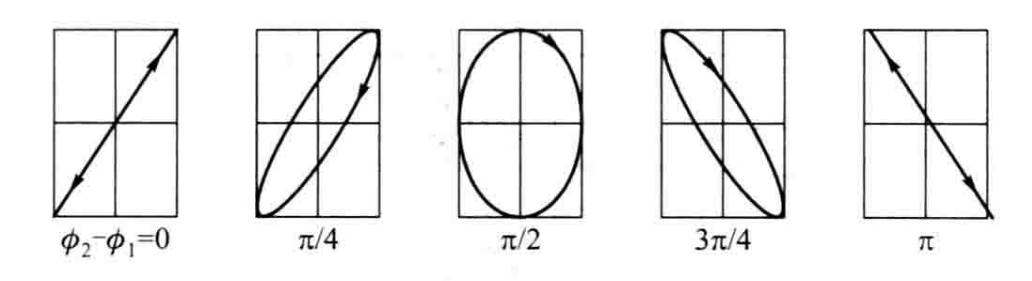
\includegraphics[width=0.8\textwidth]{figures/波形.png} 
            \caption{李萨如图形与相位差的关系}
            \label{fig:left}
    \end{figure}

    \subsubsection*{实验内容}

    \textbf{系统调节：}实验时，只有信号频率与两个具有相同固有频率的换能器频率一致时，同时只有发射端面与接收端面相平行时，才能保证良好的实验效果。调节方法：使移动端和固定端尽量靠近并平行，将接收端信号输入示波器。在信号发生器上调节频率旋钮选择谐振频率（约 40KHZ），然后微调信号发生器的频率旋钮，直至示波器上出现波幅最大为止。此时，显示的频率数值才是实验时所需的谐振频率。 
    
    \textbf{驻波法测量声速：}调节超声换能器至最佳状态后，将移动接收端来回移动，观察干涉现象。缓慢移动接收端，使示波器上出现最大的振幅波形，从标尺上读得此时的位置读数 $L_1$，继续向同一方向移动接收端，逐次记录相邻最大振幅的位置 $L_i$，连续记录12个数据，同时记下 $f$。 
    
    \textbf{相位差法测量声速：}将发射端的信号输入示波器X轴，这样发射端与接收端的振动信号分别输入示波器的X、Y轴偏转板上；在屏幕上显示了合成后的李萨如图形。移动接收端就可以在示波器上看到一、三象限的直线，从标尺上读得此时的位置读数 $L_1$，再继续移动接收端，测得示波器上看到二、四象限的直线，在标尺上读得此时的位置读数 $L_2$，连续记录12个数据。 
    
    \subsection{实验重点}

    \xiaosi（简述本实验的学习重点，不超过100字，3分）


    \begin{enumerate}   
        \item 了解声波的特性，加深对振动合成和波动干涉理论的理解；
        \item 学会用相位差法和驻波法测定声波在空气中传播的速度；
        \item 学习示波器和信号发生器的使用。
    \end{enumerate}  
    
    
    \subsection{实验难点}
    
    \xiaosi（简述本实验的实现难点，不超过100字，2分）

    \begin{enumerate}    
        \item 在使用相位比较法时，需要通过肉眼判断李萨如图形是否变为一条严格的直线。由于空气扰动会造成图形不稳定无法定格，容易引入误差 。
        \item 在使用驻波法时，示波器上的振幅在最大值（共振点）附近的变化往往不明显，存在一个较宽的“最大值区间”。判断到底哪一点是真正的峰值具有较强的主观性，容易造成较大的测量误差 。
        \item 为了消除螺旋测微机构的空程误差，移动接收端换能器时必须严格沿着同一方向旋转。如果旋转过头，严禁直接反向微调，必须退回一段距离重新向同方向逼近，否则会导致读数错误 。
        \item 实验效果高度依赖于系统的调节。只有当信号频率与换能器的固有频率严格一致（谐振），且发射端面与接收端面保持平行时，示波器上的波形幅值才最大，实验效果才好。调节频率和寻找平行的过程需要细致操作。
    \end{enumerate} 


\section{原始数据}

    \xiaosi （将有老师签名的“自备数据记录草稿纸”的扫描或手机拍摄图粘贴在下方，20分）

    \begin{figure}[htbp]
        \centering

            \centering
            
\includegraphics[width=0.9\textwidth]{figures/实验数据.jpg} 
            \label{fig:left}
    \end{figure}

\newpage
    
\section{结果与分析}

    \subsection{数据处理与结果}
    \xiaosi （列出数据表格、选择数据处理方法、给定测量或计算结果，30分）
    
    \

    \textbf{1.声速理论值的计算：} 从实验室的温度计中，我们读取得到 $t = 15.3^{\circ}C$。 

    由公式 $V_t = 331.45 \sqrt{1 + \frac{t}{273.15}} m/s$，可计算得到在 $t = 15.3^{\circ}C$ 条件下：
$V_t = 340.61 m/s$

\

在实验中，我们调节信号源输出信号谐振频率 $f=40.45 KHz$，用两种方法测量 $L_i$ 读数如下：

\begin{table}[htbp]
    \centering
    \caption{声速测定实验数据记录表}
    \label{tab:sound_speed_data}
    \begin{tabular}{ccc}
        \toprule
        \multirow{2}{*}{序号 $n$} & \textbf{驻波法} & \textbf{相位法} \\
        & 接收端位置 $L_1$ (mm) & 接收端位置 $L_2$ (mm) \\
        \midrule
        1  & 14.755 & 14.238 \\
        2  & 18.880 & 18.105 \\
        3  & 23.050 & 22.665 \\
        4  & 27.252 & 26.645 \\
        5  & 31.850 & 31.057 \\
        6  & 35.595 & 35.057 \\
        7  & 40.205 & 39.083 \\
        8  & 44.395 & 43.935 \\
        9  & 48.829 & 47.822 \\
        10 & 53.305 & 51.259 \\
        11 & 57.350 & 56.485 \\
        12 & 61.530 & 60.695 \\
        \bottomrule
    \end{tabular}
\end{table}

\textbf{2.驻波法数据处理：}

(1)计算各组波长 $\lambda_i$公式：$\lambda_i = \frac{2(x_{N+i} - x_i)}{N} = \frac{2(x_{6+i} - x_i)}{6} = \frac{x_{6+i} - x_i}{3}$
\begin{center}
    

$i=1$: $\lambda_1 = (40.205 - 14.755)/3 = 8.4833 \text{ mm}$

$i=2$: $\lambda_2 = (44.395 - 18.880)/3 = 8.5050 \text{ mm}$

$i=3$: $\lambda_3 = (48.829 - 23.050)/3 = 8.5930 \text{ mm}$

$i=4$: $\lambda_4 = (53.305 - 27.252)/3 = 8.6843 \text{ mm}$

$i=5$: $\lambda_5 = (57.350 - 31.850)/3 = 8.5000 \text{ mm}$

$i=6$: $\lambda_6 = (61.530 - 35.595)/3 = 8.6450 \text{ mm}$
\end{center}

(2) 计算平均波长 $\bar{\lambda}$公式：$\bar{\lambda} = \sum_{i=1}^{N} \lambda_i / N$$$\bar{\lambda}_1 = \frac{8.4833 + 8.5050 + 8.5930 + 8.6843 + 8.5000 + 8.6450}{6} \approx \mathbf{8.568 \text{ mm}}$$

(3) 计算实验声速 $v_{\text{实验}}$公式：$v_{\text{实验}} = f \cdot \bar{\lambda}$$$v_1 = 40450 \times 8.568 \times 10^{-3} \approx \mathbf{346.59 \text{ m/s}}$$

(4) 计算相对误差 $E$公式：$E = \frac{|v_{\text{实验}} - v_{\text{理论}}|}{v_{\text{理论}}} \times 100 \%$$$E_1 = \frac{|346.59 - 340.61|}{340.61} \times 100\% \approx \mathbf{1.76\%}$$

\textbf{3.相位法数据处理:} 

(1)计算各组波长 $\lambda_i$公式：$\lambda_i = \frac{2(x_{N+i} - x_i)}{N} = \frac{2(x_{6+i} - x_i)}{6} = \frac{x_{6+i} - x_i}{3}$
\begin{center}
    

$i=1$: $\lambda_1 = (40.205 - 14.755)/3 = 8.4833 \text{ mm}$

$i=2$: $\lambda_2 = (44.395 - 18.880)/3 = 8.5050 \text{ mm}$

$i=3$: $\lambda_3 = (48.829 - 23.050)/3 = 8.5930 \text{ mm}$

$i=4$: $\lambda_4 = (53.305 - 27.252)/3 = 8.6843 \text{ mm}$

$i=5$: $\lambda_5 = (57.350 - 31.850)/3 = 8.5000 \text{ mm}$

$i=6$: $\lambda_6 = (61.530 - 35.595)/3 = 8.6450 \text{ mm}$
\end{center}

(2) 计算平均波长 $\bar{\lambda}$$$\bar{\lambda}_2 = \frac{8.2817 + 8.6100 + 8.3857 + 8.2047 + 8.4760 + 8.5460}{6} \approx \mathbf{8.417 \text{ mm}}$$

(3) 计算实验声速 $v_{\text{实验}}$$$v_2 = 40450 \times 8.417 \times 10^{-3} \approx \mathbf{340.48 \text{ m/s}}$$

(4) 计算相对误差 $E$$$E_2 = \frac{|340.48 - 340.61|}{340.61} \times 100\% \approx \mathbf{0.04\%}$$





    \subsection{误差分析}
    \xiaosi （运用测量误差、相对误差、不确定度等分析实验结果，20分）

    本次实验中，使用驻波法相对误差为 1.76\%，相位差法为 0.04\%。分析误差来源如下：
    
    \begin{enumerate}
        \item \textbf{驻波法：}观察时，振幅在最大值附近变化不明显，判断是否达到最大值具有较强的主观性，振幅在最大值附近有较大的区间都可能被判定为最大值，造成较大的测量误差。
        \item \textbf{相位差法：}判断图像是否变为一条直线也存在一定的主观性，且空气的扰动会造成波形的跳变，由此造成一定的测量误差。
        \item \textbf{信号源：}实际实验中，信号源输出信号并非一直稳定在 设定频率不变，而是存在一定的上下浮动。
        \item \textbf{读数：}使用螺旋测微仪时，读数需估读，会造成少量误差。
    \end{enumerate}   
    
    \subsection{实验探讨}
    \xiaosi （对实验内容、现象和过程的小结，不超过100字，10分）

    \myspace{1}

    本次实验，我们分别使用驻波法和相位差法进行了声速的测定，并使用逐差法进行了数据处理和相对误差计算。整体实验操作较简单。在实验的过程中，我进一步掌握了实验原理，复习了示波器的使用，提升了基本实验素养，锻炼了实验能力。

    \section{思考题}

    \xiaosi （解答教材或讲义或老师布置的思考题，10分）

    \subsubsection*{同频率两相互垂直的振动合成中，当相位差为2π的整数倍时，李萨如图形为一、三象限的直线，当相位差为π的奇数倍时是二、四象限的直线。试证明之。}

    \textbf{答：}设两个相互垂直的简谐振动方程分别为 $x = A \cos(\omega t)$ 和 $y = B \cos(\omega t + \Delta \phi)$。
    
    当相位差 $\Delta \phi = 2n\pi$ ($n=0,1,2...$) 时，$\cos(\omega t + 2n\pi) = \cos(\omega t)$，此时 $y = B \cos(\omega t)$，结合 $x$ 的方程可消去时间 $t$ 得到 $y = \frac{B}{A}x$，这是一个斜率为正的直线方程，
    因为 $A,B$ 均为正幅值，故图形经过原点且位于第一、三象限；
    
    当相位差 $\Delta \phi = (2n+1)\pi$ ($n=0,1,2...$) 时，$\cos(\omega t + (2n+1)\pi) = -\cos(\omega t)$，此时 $y = -B \cos(\omega t)$，消去时间 $t$ 得到 $y = -\frac{B}{A}x$，这是一个斜率为负的直线方程，故图形经过原点且位于第二、四象限。   
    
    \subsubsection*{实验前为什么要调整测试系统的谐振频率？}

    \textbf{答：}实验所用的压电陶瓷换能器都有其固有的谐振频率，只有当信号发生器输出的驱动信号频率等于换能器的固有频率时，系统达到共振状态，此时电能与声能之间的转换效率最高，换能器发出的超声波强度最大，接收端转换出的电信号幅值也最大。
    
    如果频率偏离谐振点，接收到的信号会显著减弱，导致示波器上的波形振幅过小，难以准确辨别波腹（最大值）或李萨如图形的形状变化，从而增大测量误差，甚至无法进行实验。
    \subsubsection*{如果超声波发生器的频率$f =̅40.00kHz$，不确定度$u_f=10Hz$，测λ时引起波长的不确定度为$u_λ=0.03mm$ ， $λ ̅=8.560mm$ ，则实验中所测得的声速相对不确定度$u_v/v$可达多少?}

    \textbf{答：}根据相对不确定度合成公式 $\frac{u_v}{v} = \sqrt{(\frac{u_f}{f})^2 + (\frac{u_\lambda}{\lambda})^2}$，首先计算频率分量 $\frac{u_f}{f} = \frac{10}{40000} = 2.5 \times 10^{-4}$，其平方为 $6.25 \times 10^{-8}$；
    
    其次计算波长分量 $\frac{u_\lambda}{\lambda} = \frac{0.03}{8.560} \approx 3.50 \times 10^{-3}$，其平方约为 $1.23 \times 10^{-5}$；
    
    显然波长的相对误差起主导作用。将两项平方和相加后开根号：$\sqrt{6.25 \times 10^{-8} + 1.23 \times 10^{-5}} \approx \sqrt{1.236 \times 10^{-5}} \approx 0.0035$。
    
    因此，实验中所测得的声速相对不确定度 $\frac{u_v}{v}$ 可达 $3.5 \times 10^{-3}$（或 $0.35\%$）。
\newpage

\sihao\textbf{注意事项：}
\xiaosi
\begin{enumerate}
    \item  用 PDF 格式上传“实验报告”，文件名：学生姓名+学号+实验名称+周次。
    \item  “实验报告”必须递交在“学在浙大”的本课程的对应实验项目的“作业”模块内。
    \item  “实验报告”成绩必须在“浙江大学物理实验教学中心网站”-“选课系统”内查询。
    \item 教学评价必须在“浙江大学物理实验教学中心网站”-“选课系统”内进行，学生必须进行教学评价，才能看到实验报告成绩，教学评价必须在本次实验结束后 3 天内进行。
\end{enumerate}

\vspace{1cm}
\xiaosi\centering \textbf{浙江大学物理实验教学中心制}

\end{document}